\def\MyCourse{データサイエンスコース}
\def\MySubject{R入門}
\def\MySemester{春学期}

\newcommand{\R}{\textbf{R}}
\newcommand{\RStudio}{\textbf{RStudio}}
\newcommand{\Excel}{\textbf{Excel}}
\newcommand{\cs}[1]{\textcolor{blue}{\texttt{#1}}} % Console prompt >


\subsection{\R}

\myffr

  \R とは,AT&Tベル研究所が開発した統計解析用の
  プログラミング言語(S言語)
  を参考にして作られたオープンソースの言語(R言語)を使用できる
  統計解析環境.
  \vspace{5mm}

 \begin{minipage}{0.45\hsize}
  \begin{figure}
    \centering
    
\includegraphics[width=0.3\linewidth]{logo-r}
    \label{fig:logo-r}
    \caption*{The R environment}
  \end{figure}
  \end{minipage}
  \hspace{3mm}
  \begin{minipage}{0.45\hsize}
  \begin{figure}
    \centering
    \includegraphics[width=0.3\linewidth]{r-open}
    \label{fig:r-open}
    \caption*{Microsoft R Open}
  \end{figure}
  \end{minipage}

  \vspace{5mm}
  \R により,現代統計学をほぼ網羅する広範な統計解析や
  出版物品質のグラフ描画が容易に可能となる.

  \vspace{5mm}
  Microsoft社により開発・保守されている高速版の\R も存在する.

\end{frame}

\subsection{\R パッケージ}

\myffr

  \R だけでも基本的な統計解析は可能だが,
  ユーザーの利用目的に応じて開発された\R パッケージと呼ばれる
  統計解析ライブラリをインストールすることで機能を拡張できる.
  \vspace{5mm}
  
  \R パッケージは,C/C++,Fortran,R言語で記述されており,
  当初は,欧米大学の統計学科の教員らが中心となり
  開発・保守を行っていたが,
  近年は民間を含む様々な分野で広く開発が進められている.
  すでに,1,000を超える\R パッケージがインターネット上で公開されている.

\end{frame}

\subsection{CRAN}

\myffr

  CRAN(包括的R保存庫網)とは,\R の本体やパッケージ,
  マニュアル類が無償公開されているウェブサイト.
  ユーザーは,最寄りのミラーサイトからソフトウェアをダウンロードする.
  %\R 関連のソフトウェアをダウンロードする際には,
  %次の国内のサイトを利用する.

  %$\rightarrow$ 統計数理研究所(\url{https://cran.ism.ac.jp})

  \begin{figure}[h]
    \centering
    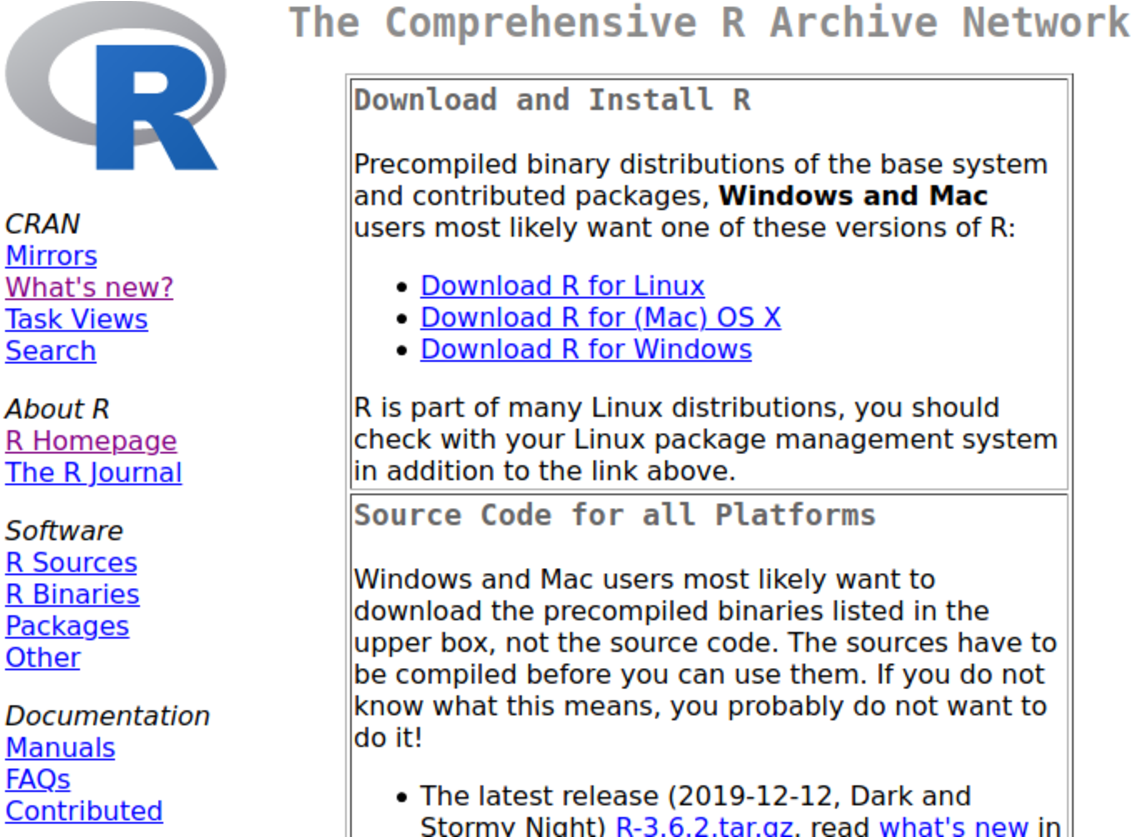
\includegraphics[width=0.6\linewidth]{cran}
    \label{fig:cran}
  \end{figure}

\end{frame}

\subsection{RjpWiki}

\myffr

  日本語での\R の情報源としては,次のウェブサイトが有名\\
  多くの有用な情報が掲載されており,質問もできる.\\
  $\rightarrow$ RjpWiki(\url{http://www.okadajp.org/RWiki})

  \begin{figure}[h]
    \centering
    \includegraphics[width=0.9\linewidth]{rjpwiki}
    \label{fig:rjpwiki}
  \end{figure}

\end{frame}

\subsection{\RStudio}

\myffr

  \RStudio とは,\R 用の統合開発環境(IDE)で,
  ソースコードの編集,実行,ヘルプの表示,パッケージの作成など,
  プログラミングに必要な様々な便利な機能を持つソフトウェア
  \vspace{3mm}
  \begin{minipage}{0.45\hsize}
    \begin{figure}[h]
      \centering
      
\includegraphics[width=0.8\linewidth]{logo-rstudio}
      \label{fig:logo-rstudio}
    \end{figure}
  \end{minipage}
  \hspace{3mm}
  \begin{minipage}{0.45\hsize}
    \begin{figure}[h]
      \centering
      \includegraphics[width=0.9\linewidth]{rstudio}
      \label{fig:rstudio}
    \end{figure}
  \end{minipage}

  \vspace{5mm}
  オープンソース版の\RStudio を次のサイトからダウンロードできる. 
  $\rightarrow$ rstudio.com(\url{https://rstudio.com})

\end{frame}

\include{def/footer}
